\documentclass[10pt]{article}

% Lines beginning with the percent sign are comments
% This file has been commented to help you understand more about LaTeX

% DO NOT EDIT THE LINES BETWEEN THE TWO LONG HORIZONTAL LINES

%---------------------------------------------------------------------------------------------------------

% Packages add extra functionality.
\usepackage{
	times,
	graphicx,
	epstopdf,
	fancyhdr,
	amsfonts,
	amsthm,
	amsmath,
	algorithm,
	algorithmic,
	xspace,
	hyperref}
\usepackage[left=1in,top=1in,right=1in,bottom=1in]{geometry}
\usepackage{sect sty}	%For centering section headings
\usepackage{enumerate}	%Allows more labeling options for enumerate environments 
\usepackage{epsfig}
\usepackage[space]{grffile}
\usepackage{booktabs}
\usepackage{amsmath}
\usepackage[super]{nth}
\usepackage{array}

% This will set LaTeX to look for figures in the same directory as the .tex file
\graphicspath{.} % The dot means current directory.

\pagestyle{fancy}

\lhead{\YOURID}
\chead{\MyLang: Language Specification}
\rhead{\today}
\lfoot{CSCI 334: Principles of Programming Languages}
\cfoot{\thepage}
\rfoot{Spring 2022}

% Some commands for changing header and footer format
\renewcommand{\headrulewidth}{0.4pt}
\renewcommand{\headwidth}{\textwidth}
\renewcommand{\footrulewidth}{0.4pt}

% These let you use common environments
\newtheorem{claim}{Claim}
\newtheorem{definition}{Definition}
\newtheorem{theorem}{Theorem}
\newtheorem{lemma}{Lemma}
\newtheorem{observation}{Observation}
\newtheorem{question}{Question}

\setlength{\parindent}{0cm}
%---------------------------------------------------------------------------------------------------------

% DON'T CHANGE ANYTHING ABOVE HERE

% Edit below as instructed
\newcommand{\MyLang}{G$\flat$}
\newcommand{\PartnerOne}{Ezra Joffe-Hancock}
\newcommand{\PartnerTwo}{Zach Stein-Perlman}
\newcommand{\YOURID}{\PartnerOne{} + \PartnerTwo{}}


\title{\MyLang: Language Specification}
\date{Spring 2022}
\author{\PartnerOne{} and \PartnerTwo{}}

\begin{document}
\maketitle

\vspace{\baselineskip}

\section{Introduction}

I (Ezra) play alto sax in a jazz combo here, and when I'm struggling with soloing over certain songs, it helps me to run over the chord changes and play along with the recording, but the best is when there's a backing track on YouTube, so I can play along with the chords without drowning whoever is soloing on the recording. I'm imagining a program that would make it easy to quickly create a backing track to play over. I imagine that you'd have to define what instrument are playing, write chords and their duration/order, set the tempo and define the length of one chorus of the song. The output would be a simple chart with the chord names along a musical bar notation of the song, and ideally a matching audio output (that keeps looping).

\section{Design Principles}
    Simple, accessible for a non-technical user. Try to make the syntax match normal English sentences and have built in functions and support for common musical terminology. Order of commands creates an easily readable layout. Prioritize simplicity over number of available features. If needed, we may rely on pure frequency sounds as notes if they are easier to produce than using looped recordings of real instruments. The written program is ideally easy to read and understand quickly what it contains as a simple piece of music.

\section{Example Programs}

Example 1:
\begin{verbatim}
  start Chorus (bars 12, volume 100, tempo 120)
      for bars(1,4):
          piano (Cmin7)
          guitar (Cmin7)
      for bars(5,8):
          piano (F7)
  end Chorus
  
  play Chorus 1
\end{verbatim}

Example 2:
\begin{verbatim}
  start Intro (bars 1, volume 60, tempo 100)
      for bars(1,1):
          piano (Gmaj)
  end Intro
 
  play Intro 1
\end{verbatim}

Example 3:
\begin{verbatim}
  start Chorus (bars 3, volume 100, tempo 144)
      for bars(1,3):
          piano (Cmaj)
  end Chorus
  
  play Chorus 4
\end{verbatim}

\section{Language Concepts}
    In order to program in the language, a user should understand the sounds/names of different instruments, have a basic understanding of chords (so they can specify them by writing out their letters), an understanding of a bar/measure which is a grouping of several beats of music. They should understand also how to transfer information from a written piece of sheet music with chords to information within the language, by copying down chords and putting them loops for the appropriate bars. We hope to also provide specifiers like volume, and tempo, so a user should understand how those qualities would affect the output. 


\section{Syntax}

    The syntax of the language is roughly as follows:
    
    We envision the largest grouping being a song, composed of several sections of music. These sections are named by the user, and when defined the user also defines the number of beats in a bar, the number of bars in the section, and the section's starting volume and tempo. The "start \textless sectionName \textgreater" command allows the users to indicate the start of a section, and the end of the section must be indicated by an accompanying "end \textless sectionName \textgreater " command. The content of the bars is specified by "for" loop declarations, the conditions of which are a range of bars, and the content of which are sound instructions. A sound instruction is composed of instruments, and what they are playing at that moment. For certain instruments, this might be chords, for others such as drums it might a selected type of beat from a limited number of options. The "and" keyword allows a set of instructions (either chord/note or a set volume/tempo) to be applied to a series of specified instruments rather than one. Each sound instruction should be on a different line within the for loop. Chords are composed of notes, but this abstraction is not revealed to the user, so that they can simply type the name of the chord and have the correct output. If a note name is accompanied by a chordal quality, such as maj, 7, min, etc. then it represents a chord. If it has no such specifier, then it represents an individual note and the instrument will make the sound accordingly. There are also the set command, which allows users to define values like the volume and tempo within a sound instruction, should they wish to change it. At the end of the program, the play function allows the user to specify the order in which the sections should be played, as well how many times. 

\section{Semantics}
\begin{enumerate}[i]
    \item What are the primitive kinds of values in your system? One kind of primitive value in our language are notes, which are of type char and are later converted using some sort of dictionary structure into either floats representing note frequencies, or directly to audio samples. Another primitive are integers, which are used to define the values of volume, tempo, bars range, and number of repeats of sections. Chords are a primitive and are a list of notes, and are created by interpreting a the name of a chord into its component notes according to some function that operates according to the rules of music theory. Instruments are primitives that are strings that represent different types of sound, they are probably matched to entries in a dictionary of dictionaries that contain audio files representing notes. Volume and tempo are primitives that are of type integer and are tied to a volume level in the output and the speed at which the audio files are played, respectively. Sound instructions are a tuple of an instrument and a chord. A sequence is a tuple of (a tuple of ints that represent the start and end bars) and a list of sound instructions. Sections are a 5-tuple of a string representing their name and an int representing the number of bars in the section and an int representing the volume level and an int representing the tempo and a list of sequences. 

    \item What are the “actions” or compositional elements of your language? In other words, how are
values combined? 
    As sort of outlined above, Instruments and chords are combined into sound instructions, which are in turn combined in sequences which follow the syntax of 
    "for bars(start: int, end: int) 
        1 or more <sound instruction>"
    
    Sections are marked by a "start \textless sectionName \textgreater" command and then a series of indented sequences until the "end \textless sectionName\textgreater" command is reached. These sections are then given as input to the play function, which produces the output of a sections (a sound or audio file) a given number of times.
    
    The only other thing to note is that the "and" operator can be used as an infix operator between instruments to make them both assigned the following chord in a sound instruction. The and operator will actually generate separate sound instructions for each instrument involved.
    
    \item How is your program represented? In other words, what components (types) will be used in
your AST? 
    Again sort of addressed above, but the types from the bottom up are Note of Int, Chord of Note list, Instrument of string, soundInstruction of Instrument * Chord, Sequence of Instruction list * (int * int), Section of string * (soundInstruction list).
    
    \item How do AST elements “fit together” to represent programs as abstract syntax? For the three
example programs you gave earlier, provide sample abstract syntax trees.
    
    
    
    Note: the current assumption is that we will somehow be able to play multiple sounds at once, either through some system player function (which we need to research) or through composing them as tracks in an audio file (which can then be played by a computer).
    
    \begin{figure}[htp]
    \centering
    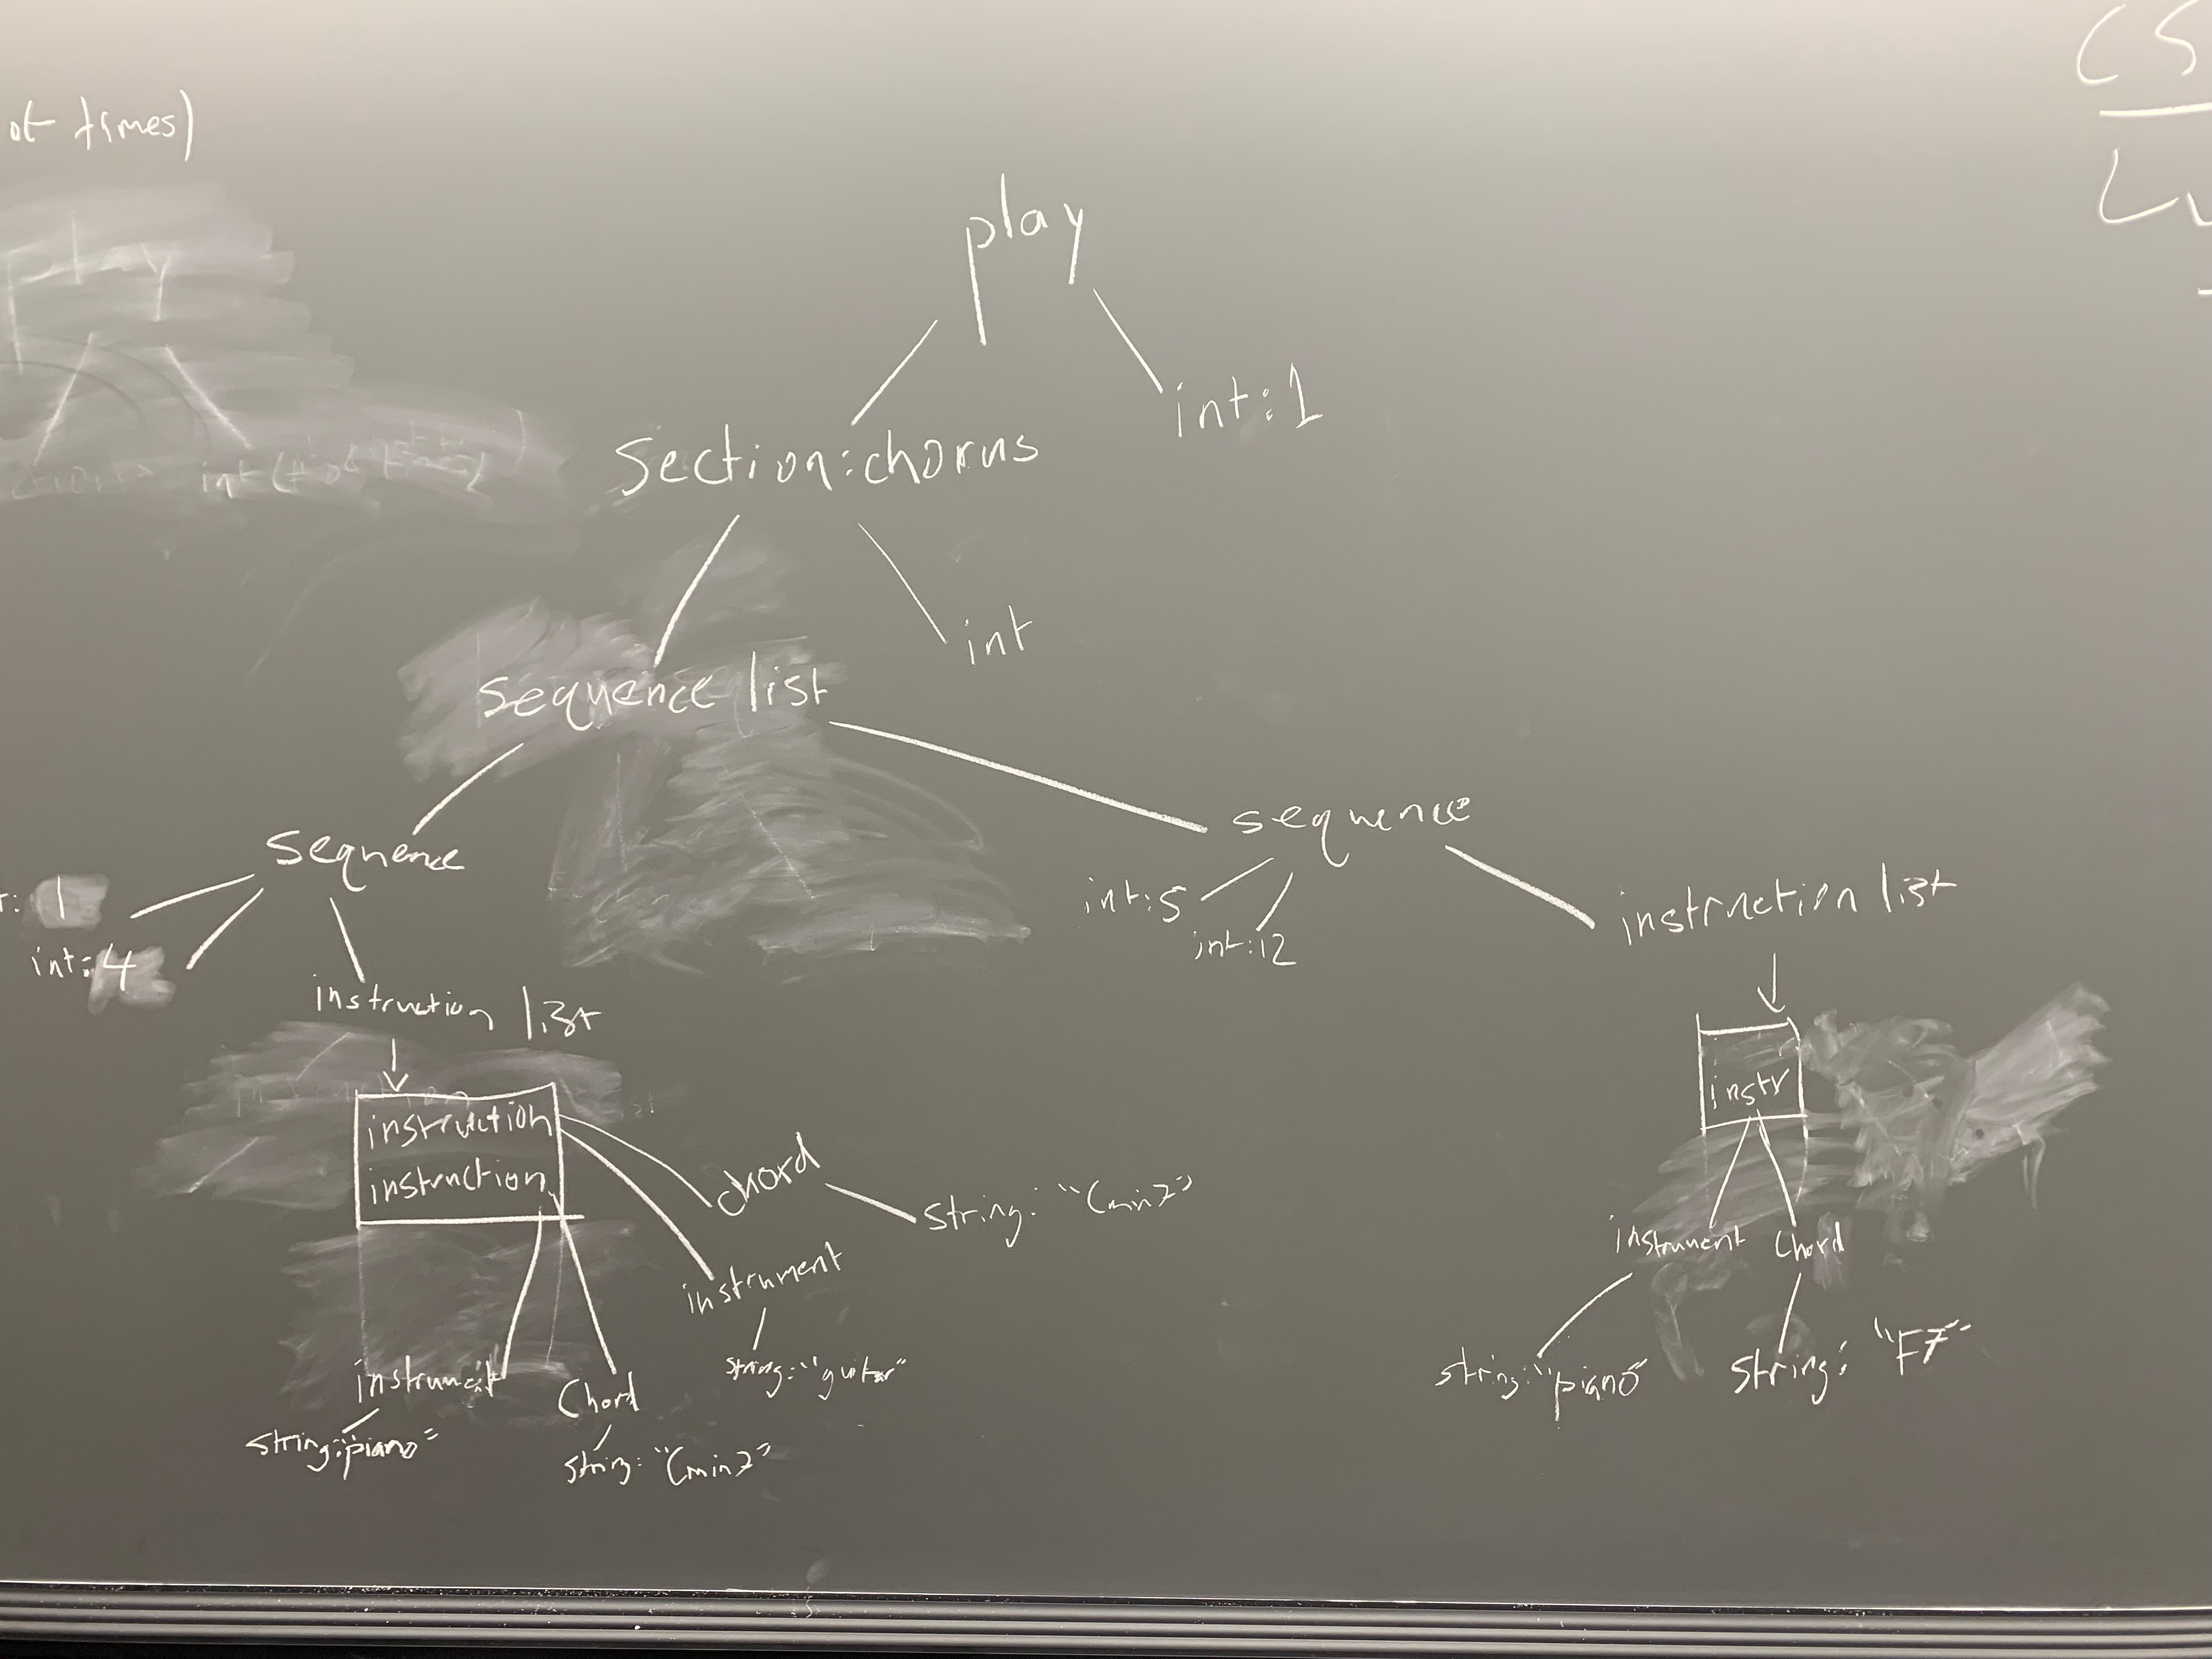
\includegraphics[width=10cm]{example1.jpeg}
    \caption{AST for example 1}
    \end{figure}
    
    \begin{figure}[htp]
    \centering
    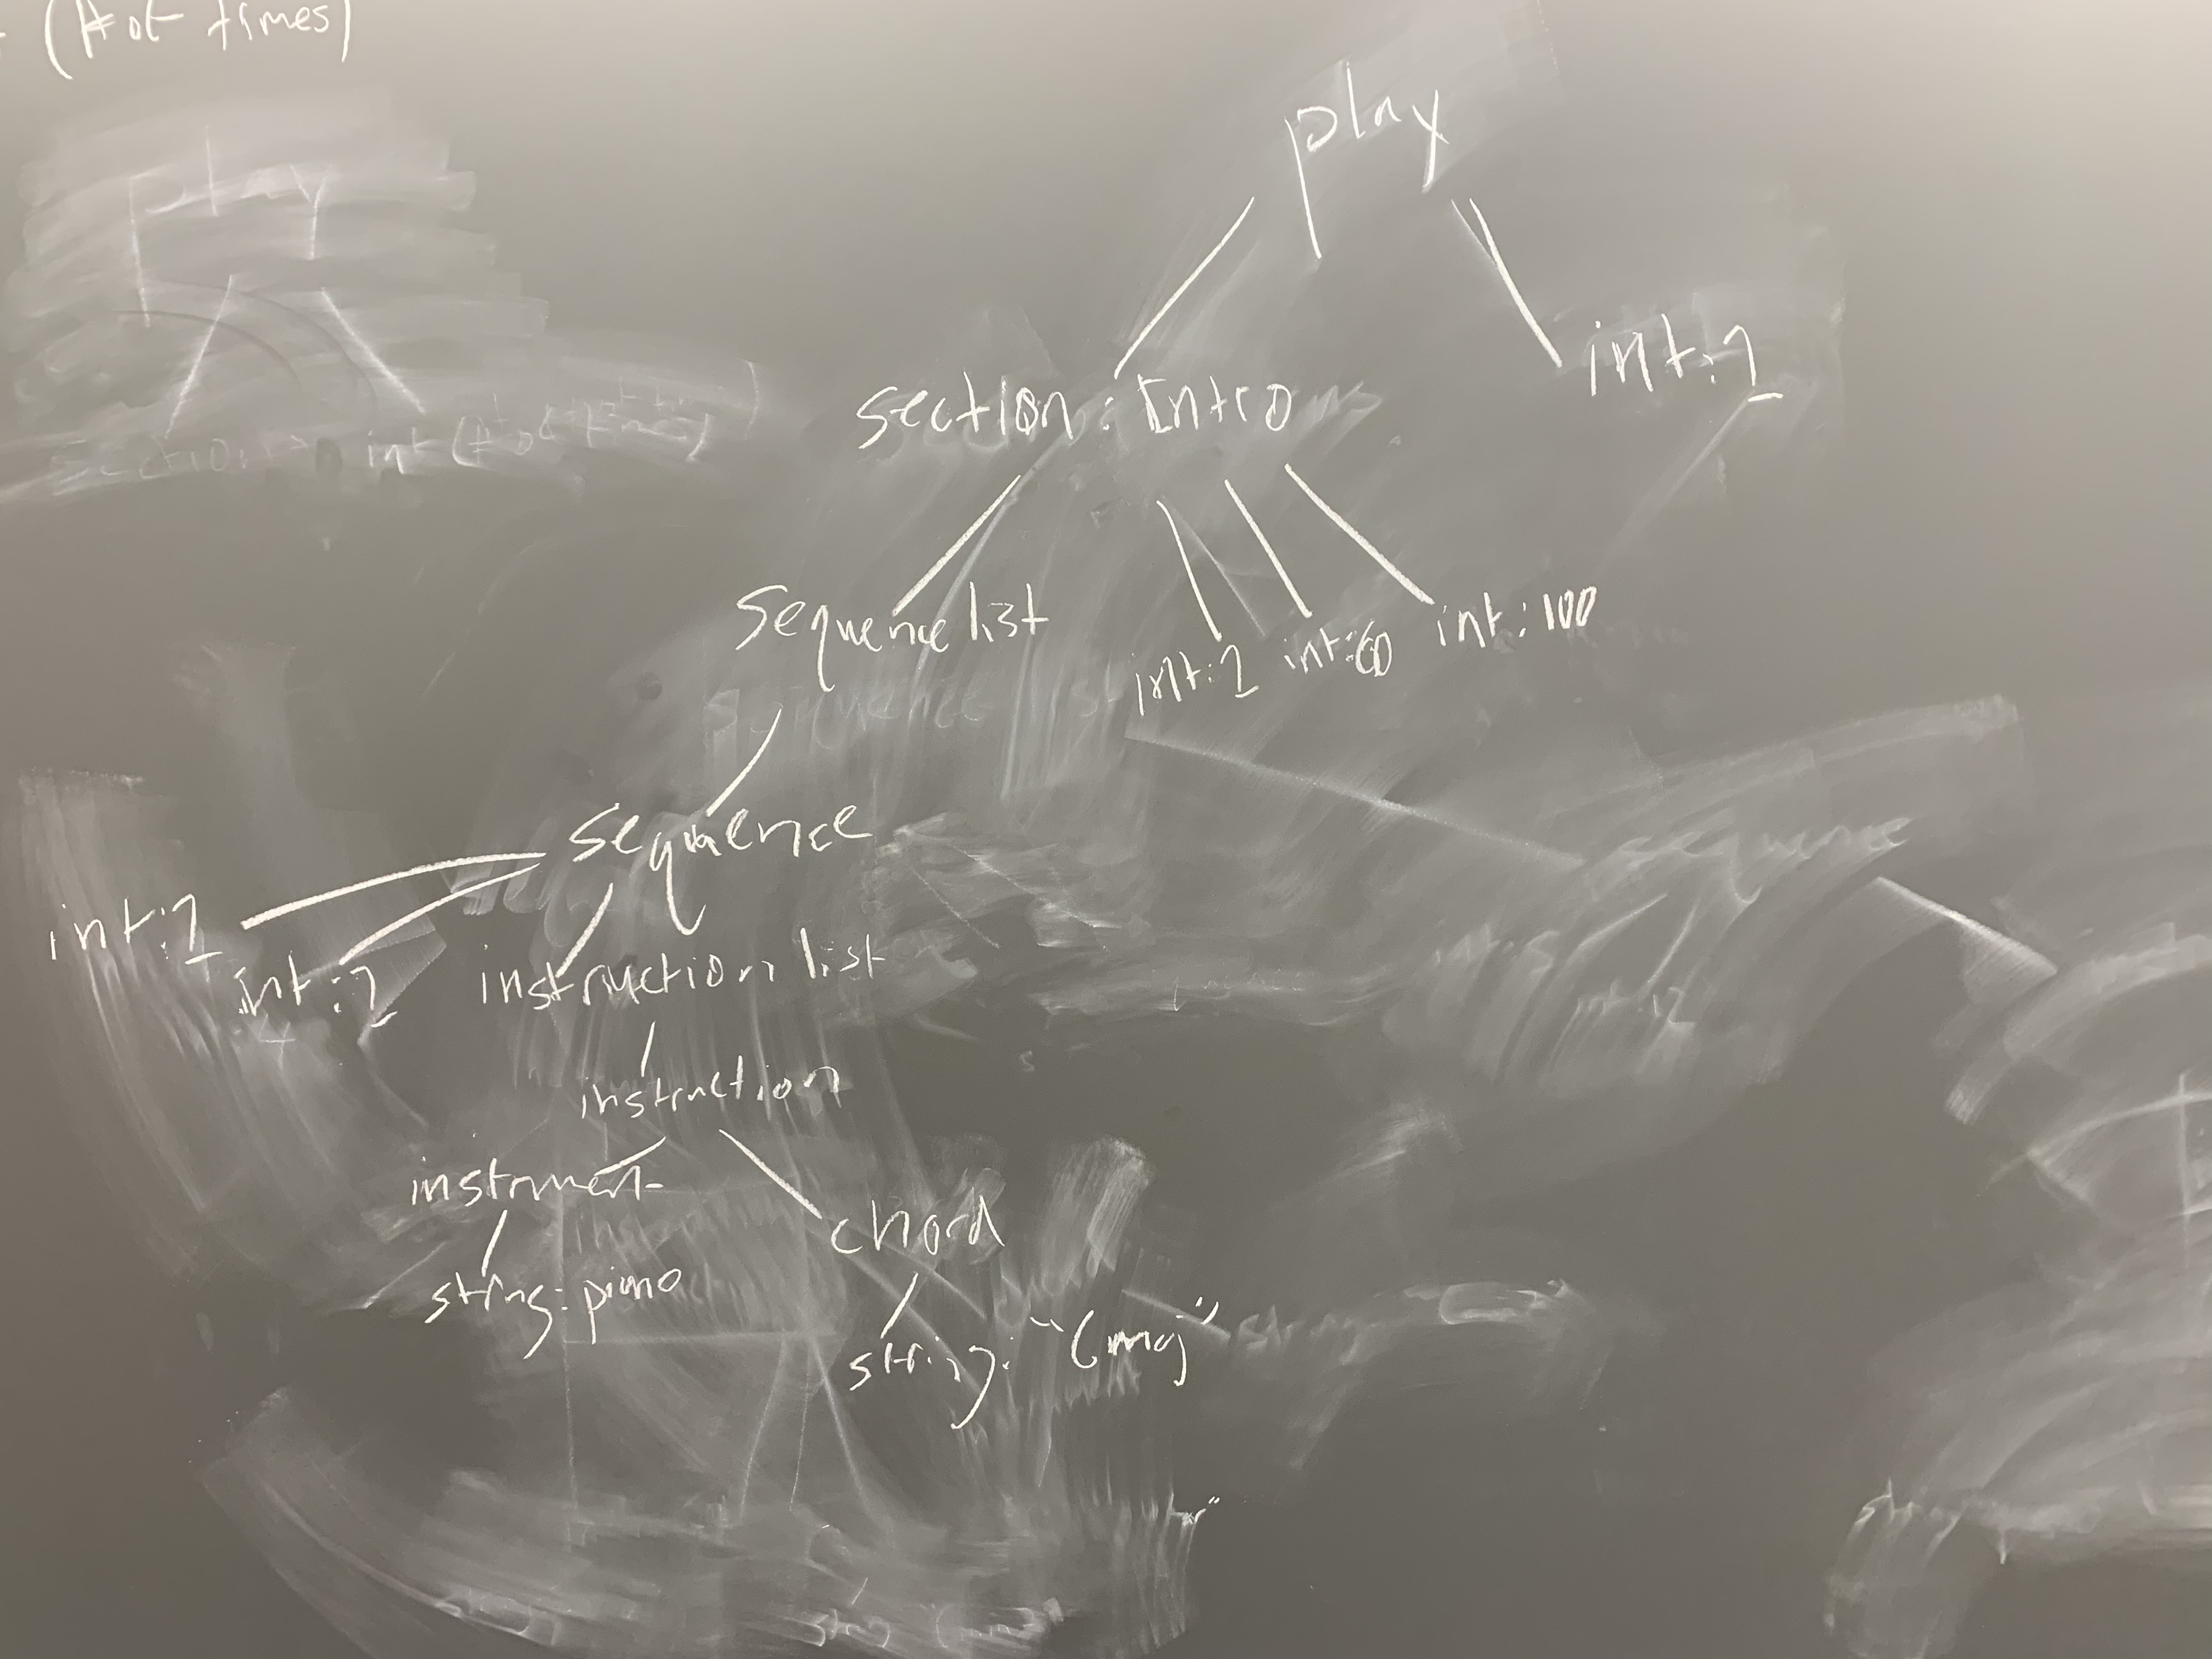
\includegraphics[width=10cm]{example2.jpeg}
    \caption{AST for example 2}
    \end{figure}
    
    \begin{figure}[htp]
    \centering
    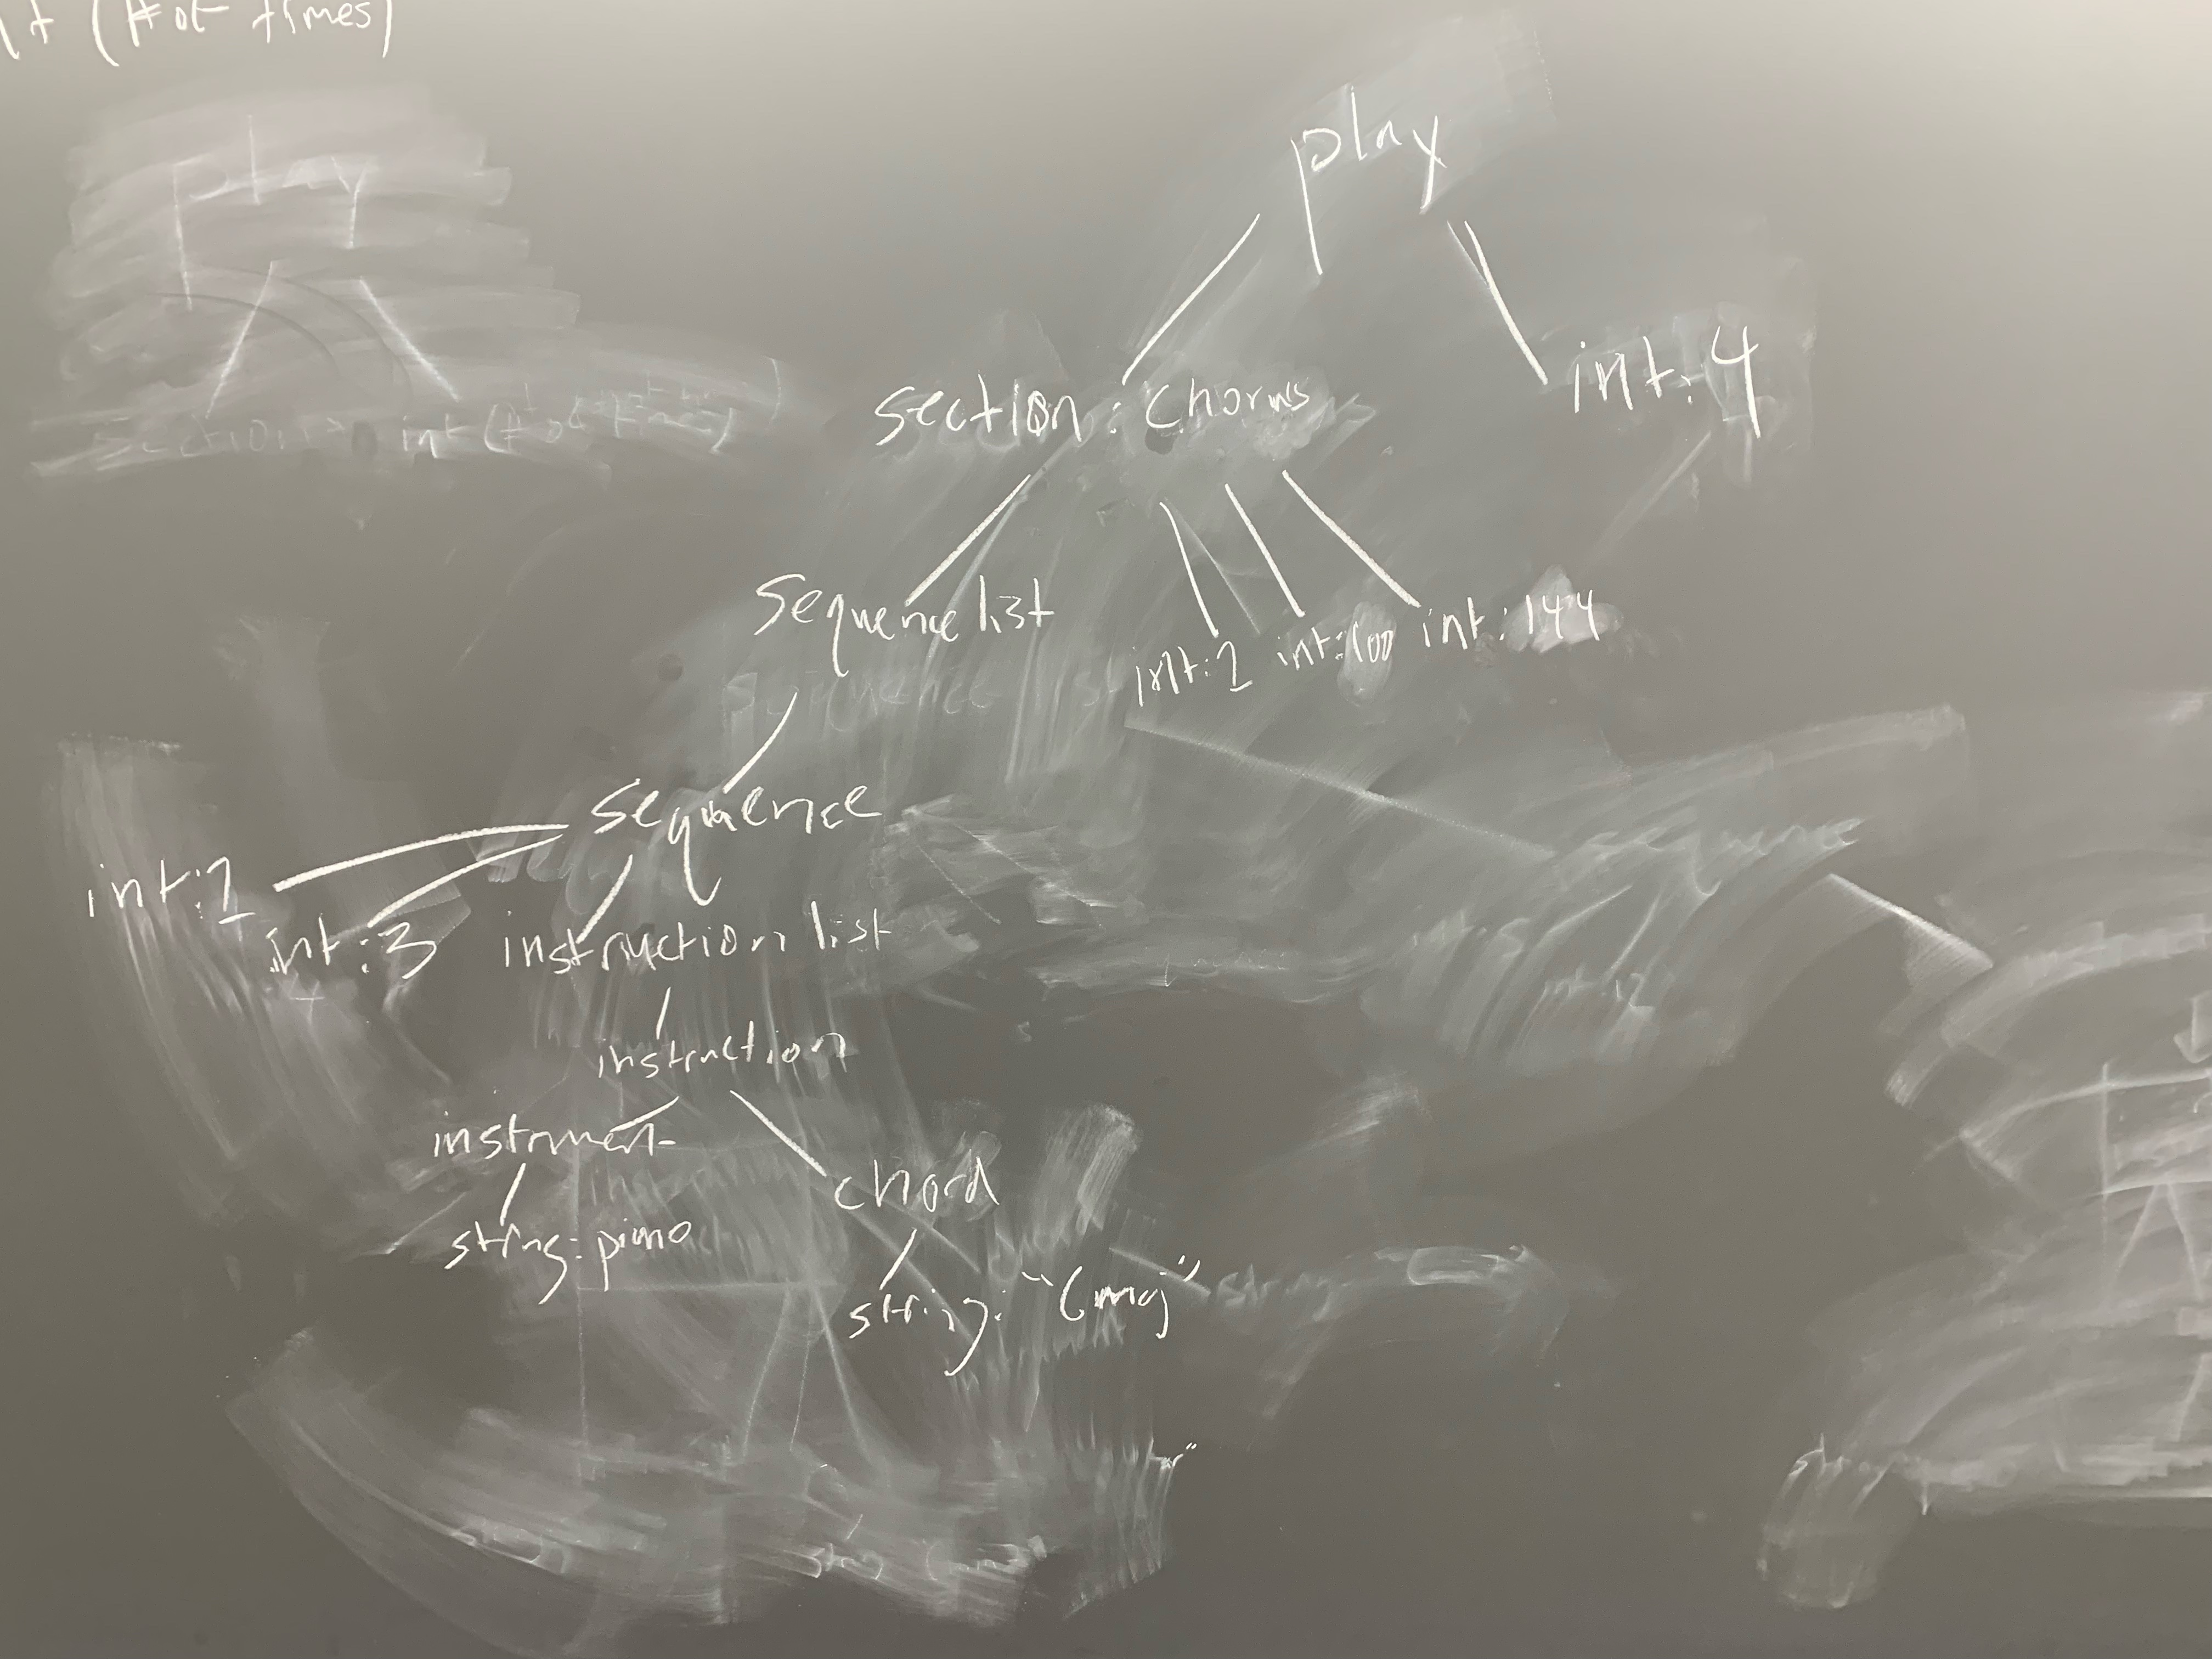
\includegraphics[width=10cm]{example3.jpeg}
    \caption{AST for example 3}
    \end{figure}
    
    \newpage\item \begin{enumerate}[A]
        \item Our programs read no input.
        
        \item Our programs output an audio file or plays sounds, not sure yet.
        
        \item Evaluation is usually conceived of as a post-order traversal of an AST. Describe how
such a traversal yields the effect you just described and provide illustrations for clarity. Demonstrate evaluation for at least one of your example programs.
    Such a traversal yields the desired structure because Chords and Instruments are paired together first in an instruction and then instructions are assembled into a sequence and then sequences fit within sections and sections are "enacted" by the play function which takes the int that represents the number of times a section should be played, only once that section has been defined through all the sub evaluations.
    
    
    
    \begin{figure}[htp]
    \centering
    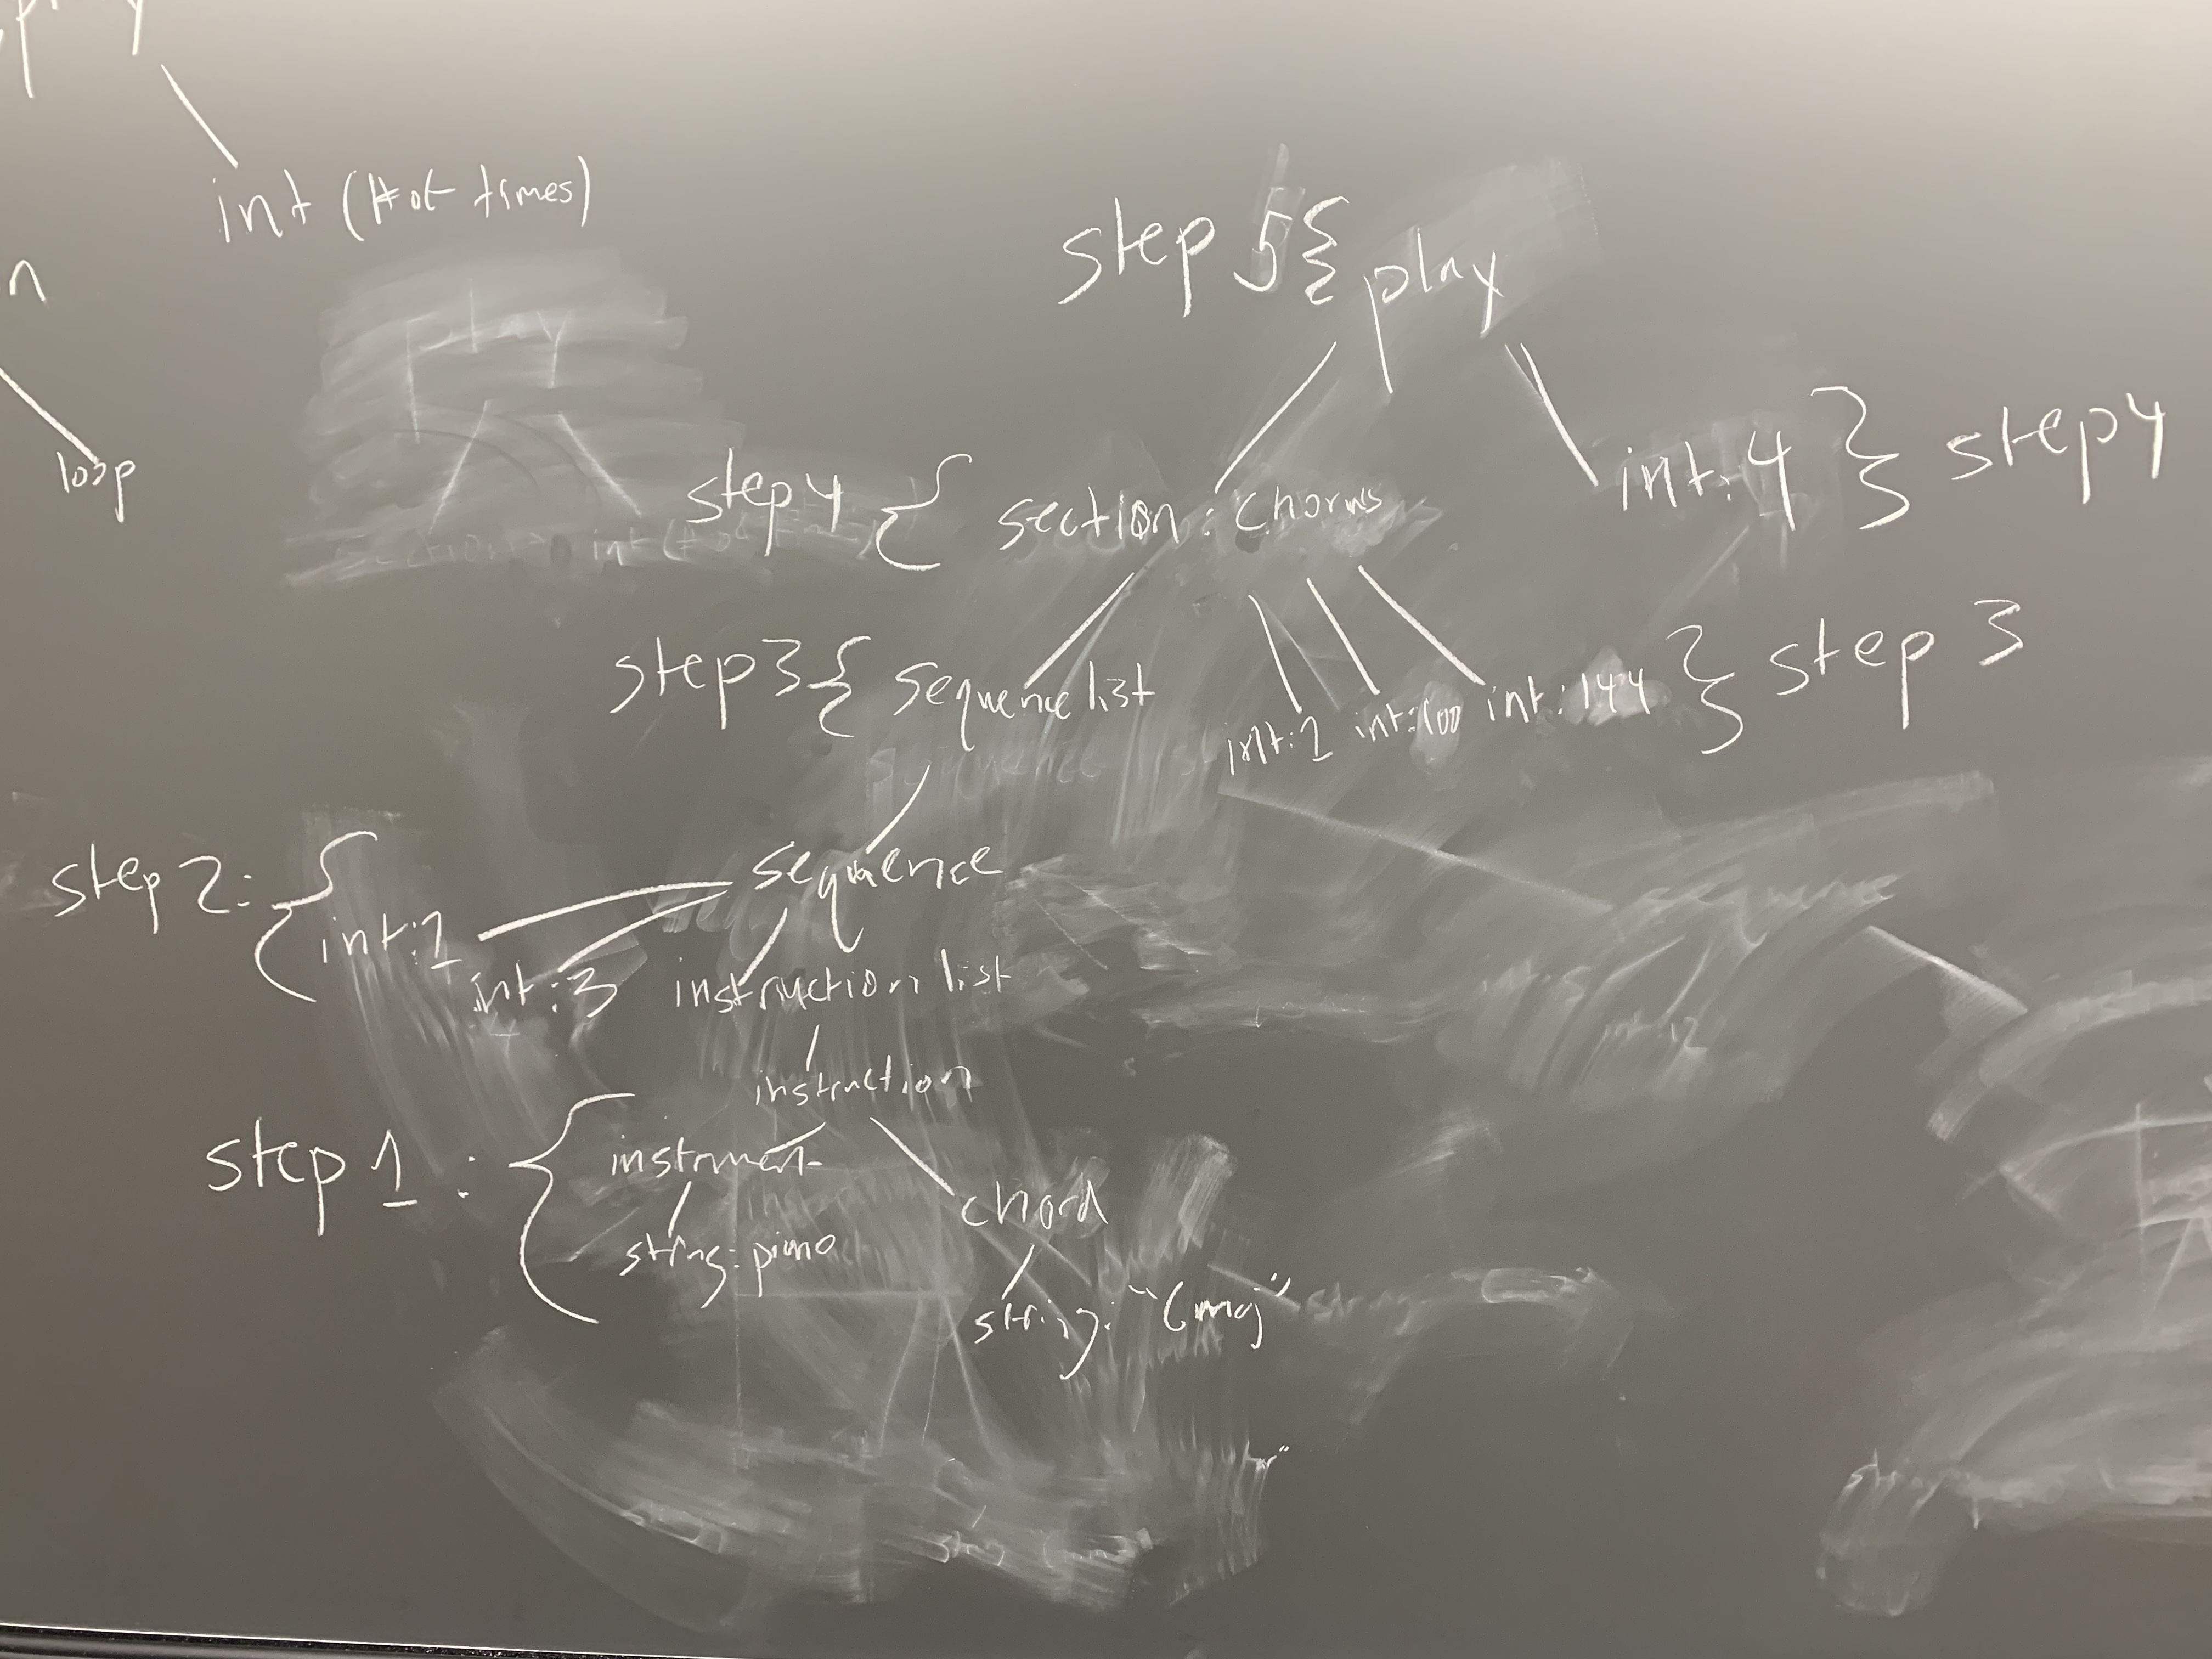
\includegraphics[width=10cm]{evaluationOrder.jpeg}
    \caption{Evaluating AST for example 3}
    \end{figure}
        
    \end{enumerate}

\end{enumerate}

% DO NOT DELETE ANYTHING BELOW THIS LINE
\end{document}
